% This work is licensed under
% http://creativecommon.org/licenses/by/3.0/
\section{Composition of the patterns}
\label{sec:sec7}

\subsection{Structural modeling}
\label{sec:structural}

The geomorphic view of networking is rigorously defined and can
be formalized.
We have formalized various aspects of the geomorphic view in
Alloy, which is the modeling language of the Alloy 
Analyzer \cite{alloy-book},
and in Promela, which is the modeling language of the Spin model
checker \cite{Spin}.
These are {\it structural models}.

Networking researchers and practitioners are accustomed to {\it analytical models},
which are also formal, but quantitative rather than structural.
One can assign numbers to some symbols in an analytical model,
give the numbers and model to a suitable evaluator, and receive
numbers for other symbols in the model.

Structural models are similar, 
except that evaluation is logical rather than quantitative.
We assume that some formulas in a model are true,
give the assumptions and the model to a suitable evaluator such
as the Alloy Analyzer or Spin,
and receive information about the truth of other formulas.
We either learn that a formula is true, or get a counterexample
showing why it is not true.

Sections~\ref{sec:sec3} through \ref{sec:sec6} should have made
clear why the term we use to describe these models is
{\it structural}.
We use them to describe hardware and software structures within
networks,
and to compare mechanisms based on where their structures are
similar and different.
We also use them to show how structural decisions constrain other
decisions and affect important properties such as scalability
and interoperability.
In the next subsection, we will mention some additional knowledge
gained with the help of structural modeling. 

\subsection{Generating the design space of mobility}
\label{sec:design}

An instance of mobility is an isolated
episode in which one layer member changes
its attachment from one underlay member to another.
One of our goals is to give network architects the freedom to handle
any instance of mobility with any mobility pattern at any level of
the layer hierarchy.
This should enhance efficiency and scalability by
allowing solutions that are finely tuned to the characteristics of
the problem they are solving.

The first step was to identify the two possible implementation patterns
and to provide sufficiently abstract versions of them
(Section~\ref{sec:sec3}).
The next step, taken in this section, is to show that any instance of
mobility can be implemented with either pattern at almost any level of
the layer hierarchy.

In the left column of Figure~\ref{fig:lift}, top half, we see a
fundamental instance of mobility in which the old and new locations
are in the same layer at Level 0.
As notated, the channel at Level 1 can be preserved by session-location
mobility (SLM) at Level 0.
In the left column, bottom half, we see a
fundamental instance of mobility in which the old and new locations
are in different layers at Level 0.
As notated, a channel at Level 2 can be preserved by dynamic routing
mobility (DRM) at Level 1.

\begin{figure}
\label{sec:fig:lift}
\centering
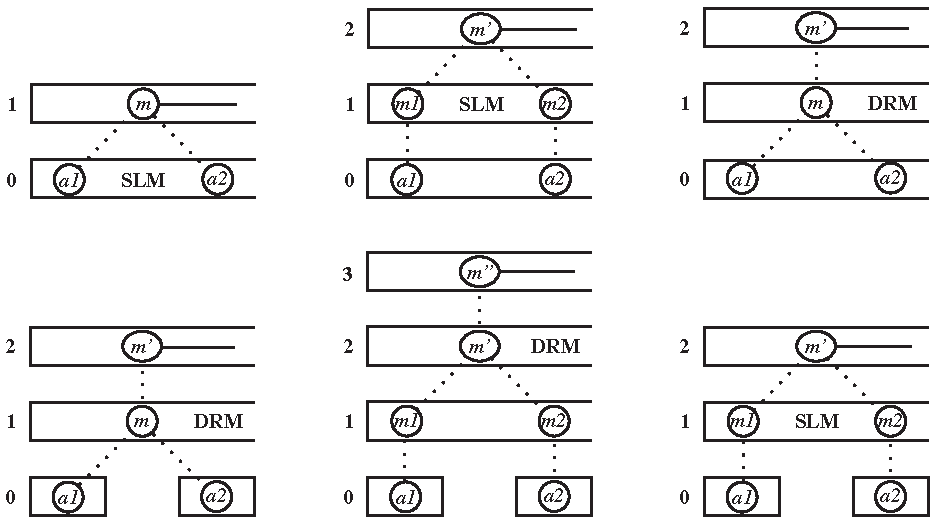
\includegraphics[scale=0.75]{figures/lift.pdf}
\caption{Generating the design space of mobility.}
\label{fig:lift}
\end{figure}

The middle column of the figure shows the effects of a ``lifting''
transformation in which each mobility implementation is moved up a level
in the hierarchy.
The purpose is to show that mobility can be implemented in many different
places, if the current architecture allows it or the designer has
control of the content and design of relevant layers.
In each case member {\it m} at Level 1 is replaced by two members
{\it m1} and {\it m2}.
Neither {\it m1} nor {\it m2} is mobile, as each has a stationary
registration in Level 0 throughout its lifetime.
Now member {\it m'} at Level 2 is mobile.
As shown in the figure (top), a channel in Level 2
with {\it m'} as its higher endpoint
can be preserved by SLM at Level 1. 
Or, as shown at the bottom, a channel in Level 3 with {\it m''} as
its higher endpoint and {\it m'} as its lower endpoint can be preserved
by DRM at Level 2.

The right column of the figure shows where one implementation pattern
can be replaced by the other.
To replace SLM by DRM (top right), it is necessary to lift the channel
up one level.
To replace DRM by SLM (bottom right), the channel can stay at the same
level, but the mobility must be lifted up a level.

Figure~\ref{fig:lift} illustrates the crucial point that mobility
is about name spaces and member identities in individual layers,
and about the mappings between these concepts in adjacent layers.
Identity is a fluid concept in software systems, which is why mobility
is fluid, and can be pushed around an architecture to appear in
different places.

If mobility is fluid, and different implementations are used for
different purposes at different levels of an architecture,
it follows that any layer could include implementations of either or
both mobility patterns.
Is this a problem?
We have proved that it is not, at least for implementations of the
patterns as modeled in Alloy.
Verification with the Alloy Analyzer shows that the two patterns
can be freely composed, in the same layer or
different layers of the same hierarchy.
They will work together without interference or other
undesirable interactions \cite{cnm}.

The limitation of this theoretical result is that,
to benefit from proven
compositionality,
implementations must maintain the minimal separation of concerns
inherent in our model of the geomorphic view.
If real implementations have state dependencies or interfering actions
that are not represented in our model, they are not necessarily
compositional even if the theorem says they are.
In effect the model is presenting sufficient
conditions for compositionality, which can be used as design guidelines
for real systems.

\subsection{Composition in Mobile IPv6}
\label{sec:mipv6}

As we saw in Section~\ref{sec:sec5}, Mobile IPv4 is an instance of DRM.
Mobile IPv6 \cite{mipv6old,mipv6new} uses a similar DRM mechanism, and
also composes it with the SLM mechanism described in 
Section~\ref{sec:sec6}.
We first consider the DRM mechanism.

Figure~\ref{fig:mipv6drm} is the Mobile IPv6 version of 
Figure~\ref{fig:mipv4}.
Note that Mobile IPv6 has no foreign agents, as their functions are
performed by the mobile hosts themselves.
In the figure, both the old attachment of {\it M} at {\it CO1}
and its new attachment at {\it CO2} are shown.
Normal routers are not shown, being replaced by ellipses in the
paths consisting of normal links.

\begin{figure}
\centering
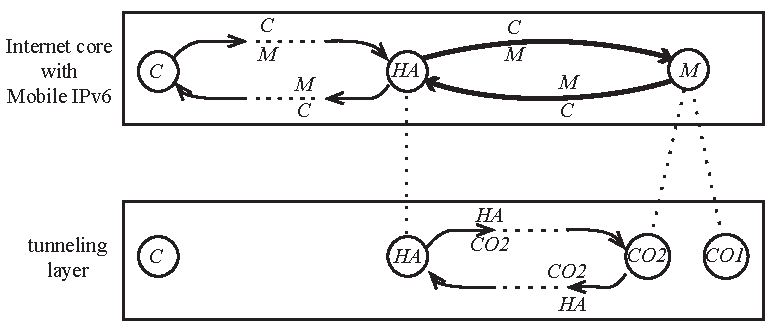
\includegraphics[scale=1.00]{figures/mipv6drm.pdf}
\caption{The paths of messages to and from mobile host {\it M} with
the dynamic-routing mobility mechanism of Mobile IPv6.
Special links are drawn with heavier lines.
Only the links employed in the path are shown.}
\label{fig:mipv6drm}
\end{figure}

Figure~\ref{fig:mipv6drm} also differs from Figure~\ref{fig:mipv4}
in showing the source and destination addresses of the messages on
every link (source on top, destination below).
Thus a message in the core layer with source {\it C} and
destination {\it M} is forwarded on a special link from {\it HA} to
{\it M}.
The implementation of this special link in the tunneling layer 
encapsulates the message in another message with source {\it HA}
and destination {\it CO2}, and sends it through normal IP links and
routers.

Figure~\ref{fig:mipv6drm} also differs from Figure~\ref{fig:mipv4}
in showing the paths of return messages from {\it M} to {\it C}.
In contrast to MIPv4, return messages from {\it M} travel on a
special link as far as {\it HA}.
At {\it HA} they enter the realm of normal links and routers.
There is no problem with ingress filtering because {\it M} belongs to
the address block of {\it HA}'s subnetwork, so {\it M} is a normal
source address at that location. 

The big problem with Mobile IP is the path cost of routing every
message through a mobile host's home agent.
Path cost is even worse in Mobile IPv6 than in Mobile IPv4, because
it is incurred by messages {\it from} a mobile host as well as
messages {\it to} it.
To reduce this problem, Mobile IPv6 standardizes a version of
SLM called ``route optimization,'' as already presented in
Section~\ref{sec:sec6}.
SLM is used only after the session between {\it C} and {\it M}
is established, and only if both endpoints have the protocol capability.

Figure~\ref{fig:mipv6slm} shows the SLM mechanism of Mobile IPv6 in
the same context as its DRM mechanism in Figure~\ref{fig:mipv6drm}.
For simplicity, this figure uses simple encapsulation as in 
\cite{mipv6old}.
After the endpoints have exchanged messages to set up SLM,
they send messages on special links implemented in the tunneling layer.
Note that these are {\it different} special links than those used
by DRM (Figure~\ref{fig:mipv6drm}).
The DRM special links involve {\it HA} and will change when {\it M}
moves.
The SLM special links do not involve {\it HA}, and will not change
from the perspective of the core layer when {\it M} moves.
With SLM, the only role played by {\it HA} in the tunneling layer is to
store the directory entry for {\it M}.
It is not needed originally because when SLM begins the two endpoints
are already connected and know each other's locations in the tunneling
layer, but it may be needed in case of simultaneous handoff.

\begin{figure}
\centering
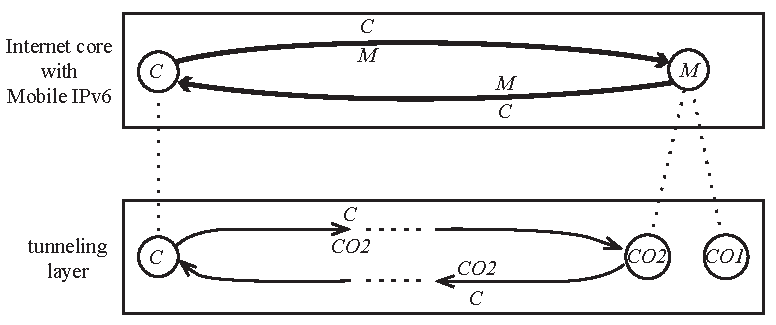
\includegraphics[scale=1.00]{figures/mipv6slm.pdf}
\caption{The paths of messages to and from mobile host {\it M} with
the session-location mobility mechanism of Mobile IPv6.
Special links are drawn with heavier lines.}
\label{fig:mipv6slm}
\end{figure}

Figure~\ref{fig:mipv6slm} also shows the SLM mechanism of Mobile IPv6
in the same context as Figure~\ref{fig:identloc}.
The ``Internet core with Mobile IPv6'' layer in
Figure~\ref{fig:mipv6slm} is the same as the identifier layer in
Figure~\ref{fig:identloc}.
The tunneling layer in
Figure~\ref{fig:mipv6slm} is the same as the locator layer in
Figure~\ref{fig:identloc}.

So far our discussion of the Internet core/identifier
layer has been limited
to its links.
We have seen that {\it C} and {\it M} may have a choice of links
over which to send their messages.
Because the network path associated with each link is different,
its performance may be different.
It is the job of TCP in the Internet core/identifier layer to
smooth over any difficulties caused by diverse paths, for example
by ensuring that messages are delivered to an application layer in
FIFO order.

The design space generated in
Section~\ref{sec:design} is intended primarily for compositions
in which different instances of mobility are managed by different
mechanisms or at different levels of the architecture.
Composition in Mobile IPv6 is a little different because the exact same
instance of mobility---pictured in the figures as {\it M}'s change
of attachment from {\it CO1} to {\it CO2}---is being handled simultaneously
by both forms of mobility.
The DRM implementation is in the core/identifier layer, while the SLM
implementation is in the tunneling/locator layer.
DRM is the default mechanism, because SLM can only be used if both
endpoints are SLM-enabled.
